\documentclass[tikz, border=5pt]{standalone}
\usepackage{amsmath}
\usepackage{amssymb}
\usepackage{tikz}
\usetikzlibrary{shapes.geometric, arrows.meta, positioning, fit, backgrounds, calc, decorations.pathreplacing}


% ── Couleurs du schéma ──────────────────────────────────────────────
\definecolor{colInput}{RGB}{70,130,180}
\definecolor{colAE}{RGB}{255,165,0}
\definecolor{colMLP}{RGB}{60,179,113}
\definecolor{colCNN}{RGB}{178,34,34}
\definecolor{colLoss}{RGB}{128,0,128}
\definecolor{colOutput}{RGB}{47,79,79}
\definecolor{colBEM}{RGB}{169,169,169}
\definecolor{colLatent}{RGB}{255,245,180}
\definecolor{colLatentBorder}{RGB}{218,165,32}
\definecolor{colLatentText}{RGB}{139,69,19}


\begin{document}

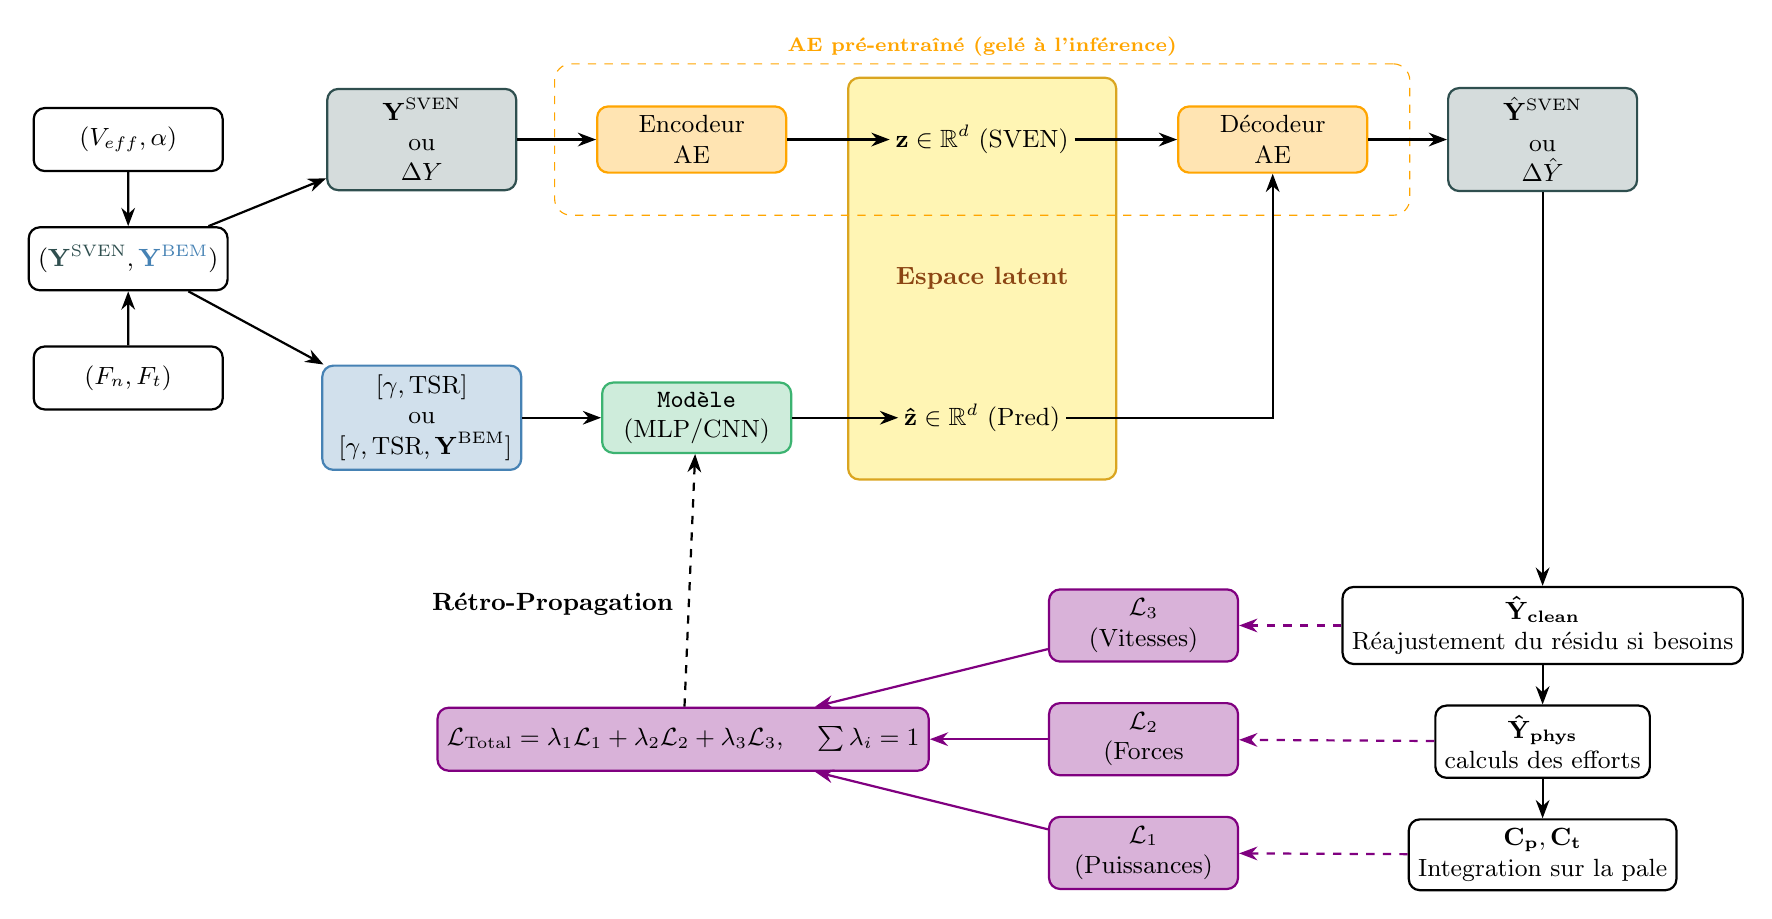
\begin{tikzpicture}[
            font=\small,
            node distance=1.2cm and 1.2cm,
            box/.style={rectangle, rounded corners=4pt, minimum width=2.4cm, minimum height=0.8cm, text centered, draw, thick, align=center},
            lat/.style={rectangle, text centered, draw=none, fill=none, inner sep=2pt},
            arrow/.style={-Stealth, thick},
            lbl/.style={font=\footnotesize\itshape, text=gray}
        ]



        %% ── LIGNE 1 : SVEN / AE ──────────────────────────
        \node[box, fill=colOutput!20, draw=colOutput] (sven_in) {$\mathbf{Y}^{\text{SVEN}}$ \\ ou \\ $\Delta Y$};
        \node[box, fill=colAE!30, draw=colAE, right= 1cm of sven_in] (enc) {Encodeur\\AE};

        \node[lat, right=1.3cm of enc] (z) {$\mathbf{z} \in \mathbb{R}^d$ (SVEN)};
        \node[box, fill=colAE!30, draw=colAE, right=1.3cm of z] (dec) {Décodeur\\AE};
        \node[box, fill=colOutput!20, draw=colOutput, right= 1cm of dec] (sven_out) {$\hat{\mathbf{Y}}^{\text{SVEN}}$ \\ ou \\ $\Delta\hat{Y}$};

        %% Bloc 0 : Input possible
        \node[box, left=1.3cm of sven_in] (v_eff) {$(V_{eff},\alpha)$};
        \node[box, below=2.2cm of v_eff] (efforts) {$(F_n,F_t)$};
        \node[label = {}](junction) at ($(v_eff)!0.5!(efforts)$) {};
        \node[box](junction) at ($(v_eff)!0.5!(efforts)$) {$(\mathcolor{colOutput}{\mathbf{Y}^{\text{SVEN}}}, \mathcolor{colInput}{\mathbf{Y}^{\text{BEM}}})$};

        %% ── LIGNE 2 : Modèle prédictif ───────────────────────────────────────
        \node[box, fill=colInput!25, draw=colInput, below=2.2cm of sven_in] (x_in)
            {$[\gamma,\text{TSR}]$\\ ou \\ $\;[\gamma,\text{TSR},\mathbf{Y}^{\text{BEM}}]$};
            
        \node[box, fill=colMLP!25, draw=colMLP, right= 1cm of x_in] (model)
            {\texttt{Modèle}\\(MLP/CNN)};

        \node[lat] (z_hat) at (z |- model) {$\mathbf{\hat{z}} \in \mathbb{R}^d$ (Pred)};
        
        % Bloc 3 : Loss et backward
        \node[box, below=5cm of sven_out] (Y_clean) {$\mathbf{\hat{Y}_{clean}}$\\ Réajustement du résidu si besoins};
        \node[box, below=0.5cm of Y_clean] (Y_phys) {$\mathbf{\hat{Y}_{phys}}$\\ calculs des efforts};
        \node[box, below=0.5cm of Y_phys] (pow) {$\mathbf{C_p}, \mathbf{C_t}$\\Integration sur la pale};

        \node[box, fill = colLoss!30, draw = colLoss, left=1.3cm of Y_clean] (L3) {$\mathcal{L}_3$ \\(Vitesses)};
        \node[box, fill = colLoss!30, draw = colLoss, below=0.5cm of L3] (L2) {$\mathcal{L}_2$\\(Forces};
        \node[box, fill = colLoss!30, draw = colLoss,  below=0.5cm of L2] (L1) {$\mathcal{L}_1$\\(Puissances)};

        \node[box, fill = colLoss!30, draw = colLoss, left=1.5 of L2] (formula) {$\mathcal{L}_{\text{Total}} = \lambda_1 \mathcal{L}_1 + \lambda_2 \mathcal{L}_2 + \lambda_3 \mathcal{L}_3$, \quad $\sum \lambda_i = 1$};

        % Ligne 0 : relier les premiers blocs aux inputs/labels
        \draw[arrow] (v_eff) -- (junction);
        \draw[arrow] (efforts) -- (junction);

         % Flèches de la ligne 1 (Horizontales)
        \draw[arrow] (junction) -- (sven_in);
        \draw[arrow] (sven_in) -- (enc);
        \draw[arrow] (enc) -- (z);
        \draw[arrow] (z) -- (dec);
        \draw[arrow] (dec) -- (sven_out);

        % Loss & Backward
        \draw[arrow] (sven_out) -- (Y_clean);
        \draw[arrow] (Y_clean) -- (Y_phys);
        \draw[arrow] (Y_phys) -- (pow);

        \draw[arrow, dashed, colLoss] (Y_clean) -- (L3);
        \draw[arrow, dashed, colLoss] (Y_phys) -- (L2);
        \draw[arrow, dashed, colLoss] (pow) -- (L1);

        \draw[arrow, colLoss] (L3) -- (formula);
        \draw[arrow, colLoss] (L2) -- (formula);
        \draw[arrow, colLoss] (L1) -- (formula);
        
        \node[above=1.3cm of formula, anchor=east] {\textbf{Rétro-Propagation}};
        \draw[arrow, dashed] (formula) -- (model); % {\textbf{Rétro-Propagation}};

        %% ── FLÈCHES ET RACCORDS ────────────────────────────────────
        \draw[arrow] (junction) -- (x_in);
        \draw[arrow] (x_in) -- (model);
        \draw[arrow] (model) -- (z_hat);
        \draw[arrow] (z_hat.east) -| (dec.south);

        %% ── BLOC JAUNE : ESPACE LATENT ─────────────────────────────────────
        \begin{scope}[on background layer]
        \node[rectangle, rounded corners=4pt,
                fit=(z)(z_hat),
                fill=colLatent, draw=colLatentBorder, thick,
                inner xsep=15pt, inner ysep=15pt] (latent_block) {};
                

        \node[font=\small\bfseries, text=colLatentText] at (latent_block.center) {Espace latent};
        \end{scope}


        %% ── ENCADRÉ GLOBAL : AE PRÉ-ENTRAÎNÉ ─────────────────
        \begin{scope}[on background layer]

        \node[draw=colAE, dashed, rounded corners=6pt, inner sep=15pt,
                fit=(enc)(z)(dec),
                label={[font=\scriptsize\bfseries, text=colAE, yshift=-1pt]above:{AE pré-entraîné (gelé à l'inférence)}}] {};
        \end{scope}

\end{tikzpicture}

\end{document}